% !TeX spellcheck = fr-moderne

\section{Des normes de téléphonie mobile}
Depuis 1984, il y a déjà plusieurs standards ont été utilisé par les opérateur dans le monde entier. Voici un tableau de différentes standards mobile en Europe et ses paramétrés \ref{tbl:GMIE}. 
\begin{table}[H]
\begin{tabular}{|p{2cm}|p{2cm}|p{2cm}|p{4cm}|}
	\hline
	Génération&Acronyme&Description&Débit\\
	\hline
	1G		&Radiocom 2000	&Échanges de type voix uniquement&analogique\\
	\hline
	\hline
	2G		&GSM			&Échanges de type voix uniquement	&9,05 kbps\\
	\hline
	2,5G	&GPRS			&Échange de données sauf voix		&171,2 kbps / 50 kbps / 17,9 kbps\\
	\hline
	\hline
	3G		&UMTS			&Voix + données						&144 kbps rurale, 384 kbps urbaine, 1,9 Mbps point fixe / -\\
	\hline
	3.5G ou 3G+ ou H&HSPA	&Évolution de l'UMTS				&14,4 Mbps / 3,6 Mbps / -\\
	\hline
	\hline
	4G		&LTE			&Long Term Evolution (Données)				&150 Mbps / 40 Mbps / -\\
	\hline
	4G		&LTE-Advanced	&Long Term Evolution Advanced (Données+voix)		&1 Gbps à l'arrêt, 100 Mbps en mouvement / - / -\\
	\hline
\end{tabular}
\caption{Les différentes générations de téléphonie mobile en Europe}
 \label{tbl:GMIE}
\end{table}
En télécommunication, \textsf{1G} est la premier génération des standards pour la téléphonie mobile, il s'agit de la première apparition du réseaux de téléphonie mobile, 1G sont des réseaux analogiques, peut échanges de type voix uniquement.

\textsf{2G}, la technologie de téléphonie sans fil de deuxième génération, la différence entre le réseaux 1G et 2G est: le signaux radio sur les réseaux 1G sont analogiques, et celle de 2G sont numériques.

Systèmes 2G ont été significativement plus efficaces du spectre permettant de bien plus grand taux de pénétration du téléphone mobile, en plus les données vocales numériques peuvent être compressées et multiplexées beaucoup plus efficacement que les codages de la voix analogique grâce à l'utilisation de codecs différents, ce qui permet plus d'appels à transmettre dans la même quantité de bande passante radio. Et 2G présenté premier foi les services de données pour mobile. Les Technologie 2G permettent les divers réseaux de téléphonie mobile de utiliser des services tels que le SMS et MMS. Tous les message de texte envoyés au delà de 2G sont chiffrés numériquement, ce qui permet le transfert de données de telle sorte que seul le destinataire peut recevoir et lire.   

Réseaux 2G ont été construits principalement pour les services téléphoniques et de transmission de données lent (défini dans les documents de spécifications IMT-2000).

Réseaux \textsf{2,5G}, on le qualifie souvent de le General packet Radio Service ou GPRS, est une norme pour la téléphonie mobile dérivée du GSM et complémentaire de celui-ci, permettant un débit de données plus élevé. Le 2,5 indique que c'est une technologie à mi-chemin entre le GSM (deuxième génération) et l'UMTS (troisième génération). Le GPRS est une extension du protocole GSM : il ajoute par rapport à ce dernier la transmission par paquets. Cette méthode est plus adaptée à la transmission des données. En effet, les ressources ne sont allouées que lorsque des données sont échangées, contrairement au mode « circuit » en GSM où un circuit est établi – et les ressources associées – pour toute la durée de la communication. Le GPRS a ensuite évolué au début des années 2000 vers la norme \textsc{edge} également optimisée pour transférer des données et qui utilise les mêmes antennes et les mêmes fréquences radio.

La troisième génération (3G) des normes de téléphonie mobile. Elle est représentée principalement par W-CDMAmm, CDMA2000, TD-SCDMA et WiMAX. Elle permettant des débits de 2 à 42 Mb/s qui sont bien plus rapides qu'avec la génération précédente. Grâce à l'utilisation des règles de classement utilisateur, et les  bandes de fréquences supérieures rendant la capacité du réseau augmenter.

La quatrième génération des standards pour la téléphonie mobile, succédant à la 2G et la 3G, en théorie, elle permet de transmette de données à des débits supérieur à 100 Mb/s. 

Une des particularité de la 4G est sa EPC (Evolved Packet Core) est basé sur IP, et il n'y a plus de mode commuté (le 'Circuit Switched Domain' qui s'occupe le service vocaux dans les standard précédant), ce qui signifie que les services vocaux transmis sur l'internet \ref{Fig.3G}. 

\begin{figure}[H]
	\centering
	\subfigure[Réseau 3G et ses predecesseur]{
		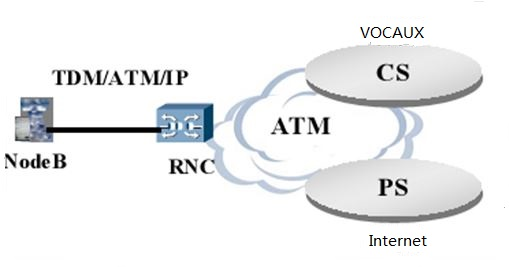
\includegraphics[width=3in]{images/3G2.JPG}}\hfill
	\hspace{1in}
%\flushright
	\subfigure[Réseau 4G]{
		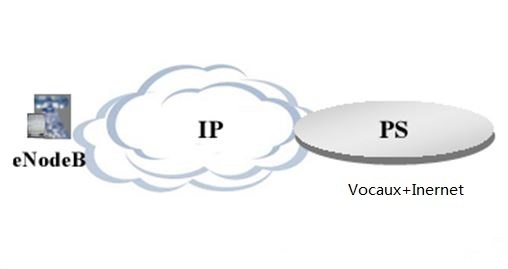
\includegraphics[width=3in]{images/4g.JPG}}
	\caption{Structure des réseaux} 
		\label{Fig.3G}
\end{figure}

Le réseau 4G contient 2 partie: eNodeB (le station), EPC (Evolved Packet Core) qui contient MME, S-GW, P-GW et HSS \ref{structure4G}.
      \begin{figure}[H]
          \centering
          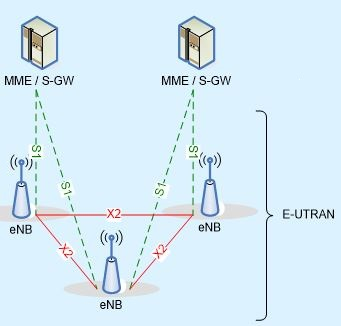
\includegraphics[width=3in]{images/enb.jpg}
          \caption{la structure du réseau}
          \label{structure4G}
      \end{figure}